\documentclass[11pt, letterpaper, openany]{memoir}

% --------------------------
% Packages
% --------------------------
\usepackage{varwidth}
\usepackage{import}
\usepackage[svgnames]{xcolor} % https://www.w3.org/TR/SVG11/types.html#ColorKeywords
\usepackage{parskip}
\usepackage{fontspec}
\usepackage{titlesec}
\usepackage{tabu}
\usepackage{url}
%\usepackage{geometry}
\usepackage{graphicx}
\usepackage{wrapfig}
\usepackage{etoolbox}
\usepackage{xstring}
\usepackage{catchfile}
\usepackage{titlesec}
%\usepackage{gitinfo2}
\usepackage{longtable}

% --------------------------
% Templates and other
\import{./templates/}{mech-template.tex}
\import{./templates/}{gear-template.tex}
\import{./templates/}{npc-template.tex}
\import{./templates/}{background-template.tex}
\import{./templates/}{talent-template.tex}

% --- always last
\usepackage[hidelinks,bookmarks=true]{hyperref}
% hypersetup, below

% --------------------------
% Configuration
% --------------------------
\setlength{\parskip}{1.0\baselineskip plus2pt minus2pt}

\setlrmarginsandblock{25.4mm}{22.2mm}{*}
\setulmarginsandblock{1in}{1in}{1}
\checkandfixthelayout

\setlength{\oddsidemargin}{0pt}
\setlength{\evensidemargin}{0pt}

\interfootnotelinepenalty=10000
\raggedright

\setmainfont{Arial}

\hypersetup{colorlinks=false
  %linkcolor=DarkBlue, % color of internal links (change box color with linkbordercolor)
  %  urlcolor=blue       % color of external links
}

% Remove empty page after title
% toto use etoolbox
\makeatletter
\renewcommand\mainmatter{%
     \clearpage
   \@mainmattertrue
   \pagenumbering{arabic}}
\makeatother

\makeatletter
\patchcmd{\chapter}{\if@openright\cleardoublepage\else\clearpage\fi}{}{}{}
\makeatother

% --------------------------
% Loading
% --------------------------
\graphicspath{ {./images/} }


% --------------------------
% Commands and Environments
% --------------------------
\providecommand{\fluff}[1]{{\itshape #1}}
\providecommand{\punch}[1]{\textbf{\Large #1}}

\newenvironment{loreQuote}
{\begin{center}
\begin{varwidth}{\textwidth}
  \small \itshape}
{\end{varwidth}
\end{center}}

\titleformat
{\chapter} % command
[block] % shape
{\bfseries\Huge} % format
{} %label
{} %sep
{\centering} % before-code
[] % after-code

\titleformat
{\section} % command
[block] % shape
{\bfseries\LARGE} % format
{} %label
{} %sep
{\centering} % before-code
[] % after-code

\titleformat
{\subsection} % command
[block] % shape
{\bfseries\Large} % format
{} %label
{} %sep
{\centering} % before-code
[] % after-code

\titleformat
{\subsubsection} % command
[block] % shape
{\bfseries\large} % format
{} %label
{} %sep
{\centering} % before-code
[] % after-code

\begin{document}
\frontmatter
\pagestyle{empty}
\pagenumbering{gobble}
\begingroup
\patchcmd{\chapter}{plain}{empty}{}{}

% Get all subsub(etc) sections to show in toc
\setcounter{secnumdepth}{-2}
\setcounter{tocdepth}{7}

%\pagestyle{empty}
\begin{center}
  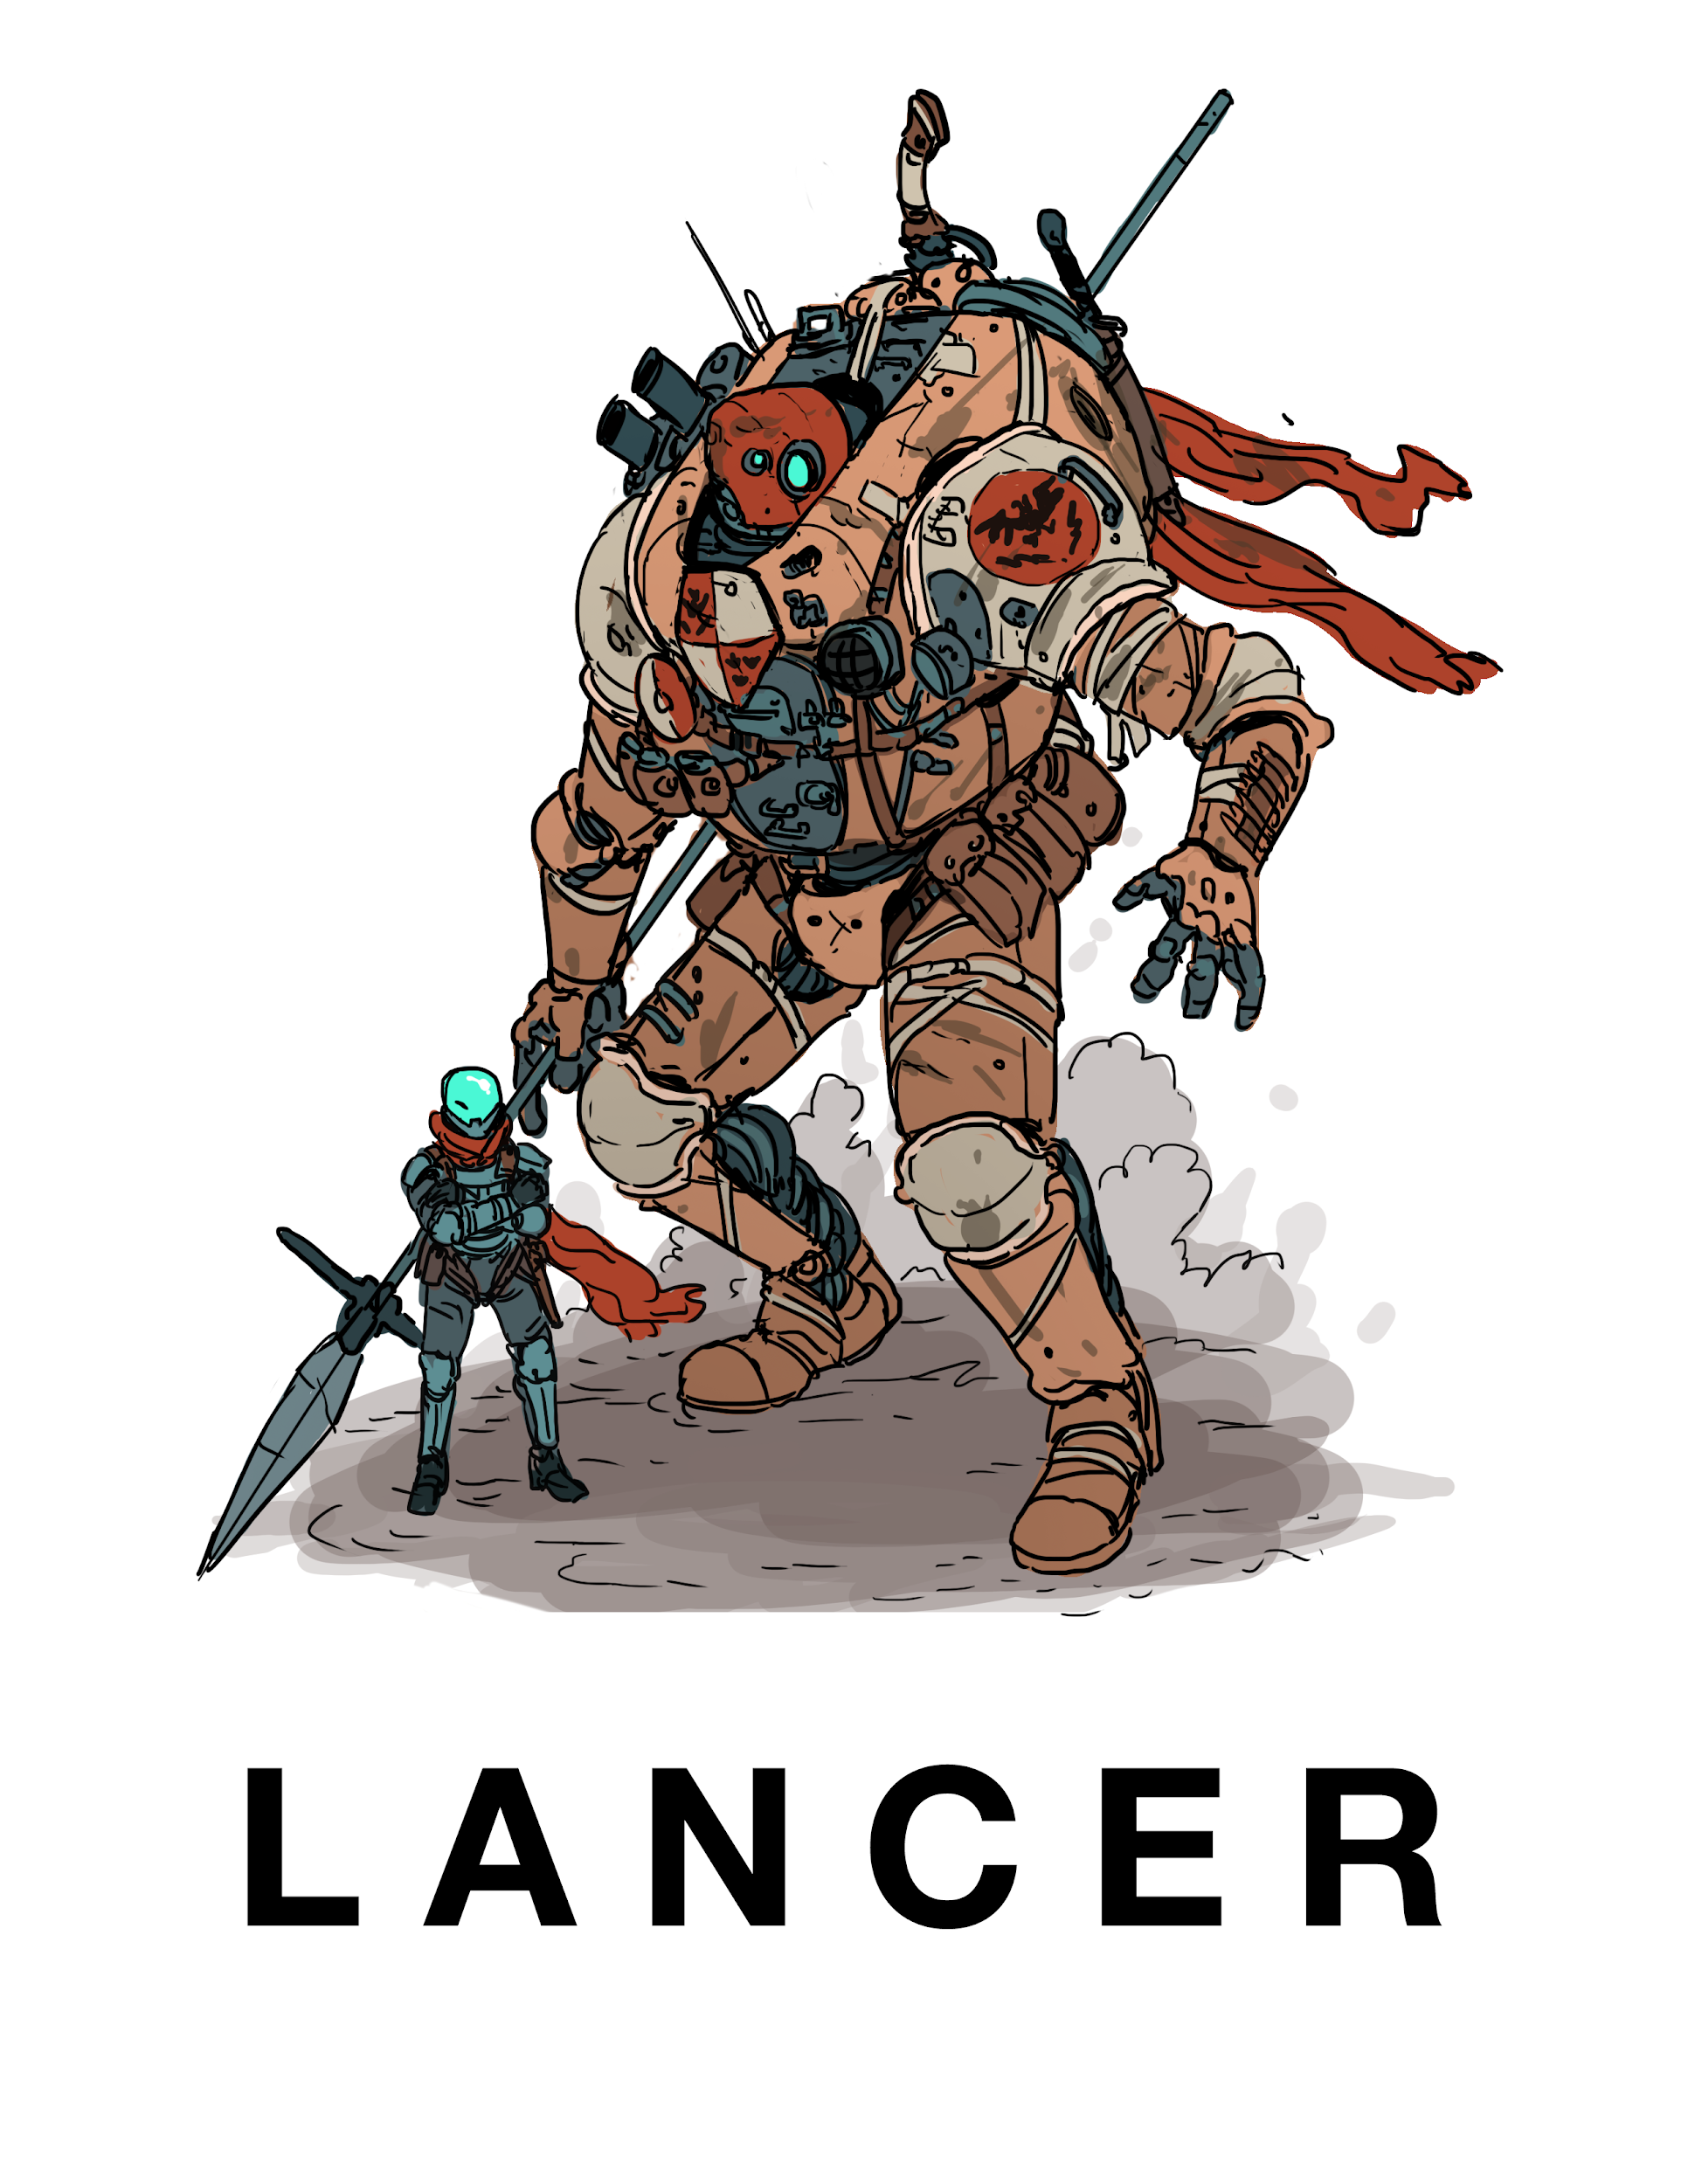
\includegraphics{Cover}
\end{center}

%\newpage
%\pagestyle{plain}
%\begin{titlingpage}
\vspace*{\stretch{1.0}}
\begin{center}
%\par\noindent\rule[1cm]{0.78\textwidth}{3mm}
\rule[1cm]{0.78\textwidth}{3mm}
{\fontsize{96}{115}\selectfont LANCER}
\rule[-1cm]{0.78\textwidth}{3mm}

\vspace{2cm}
\huge\textbf{COMMUNITY EDITION RULEBOOK}

\vspace{4cm}
\normalsize\textbf{By} \\
% TODO: add hyperlinks
\textbf{Miguel Lopez and Tom Parkinson Morgan}\\
\textbf{and the Lancer community}\\

\vspace{2cm}
\date{} % quick hack to suppress date showing on wrong page
Document generated: \today \\
%Document version: \texttt{\gitshort} on branch \texttt{\branch}
%Document version: \gitAbbrevHash \ on branch \gitBranch, committed \gitAuthorDate

\vspace{1cm}
1.8 Beta - CE pre-release\\
Please do not reproduce without permission
\clearpage
\end{center}

\import{source/}{changelog}
\clearpage

\tableofcontents
\endgroup % end of empty grounp
\mainmatter
\pagestyle{plain}
% We set the page number to 2, so the PDF page number = the text page number
% TODO: this must be automatable.
\addtocounter{page}{12}

\import{source/}{intro}
\import{source/}{cavalry}
\import{source/}{basicRules.tex}
\import{source/}{licenseToKill.tex}
\import{source/}{pilot.tex}
\import{source/}{basicStructure.tex}
\import{source/}{theMech.tex}
\import{source/}{mechCombat.tex}
\import{source/}{compendium.tex}
\import{source/}{theGM.tex}
\import{source/}{gmToolkit.tex}
\import{source/}{npc.tex}
\import{source/}{lore.tex}

\end{document}